\begin{figure}[t!]
    \centering
    \begin{subfigure}[t]{\linewidth}
        \centering
        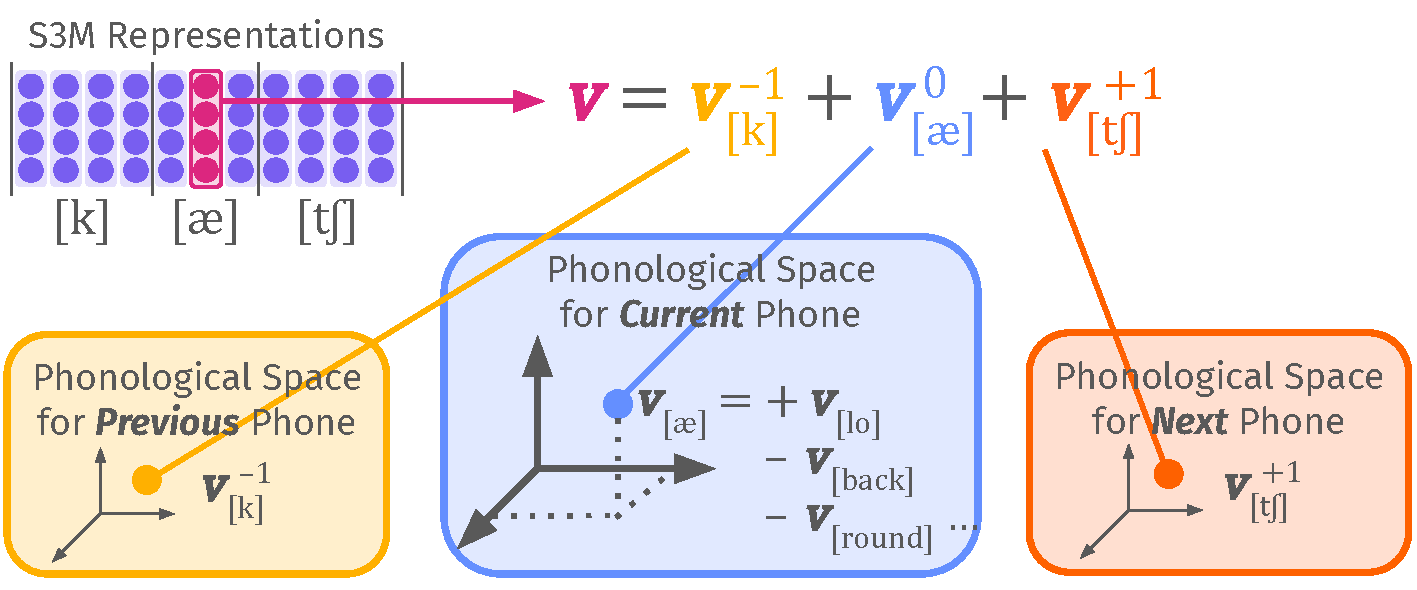
\includegraphics[width=\linewidth]{pdfs/fig1.pdf}
        \caption{
            Conceptual illustration of our hypothesis.
        }
        \label{fig:summary}
    \end{subfigure}

    \vspace{1em}

    \begin{subfigure}[t]{\linewidth}
        \centering
        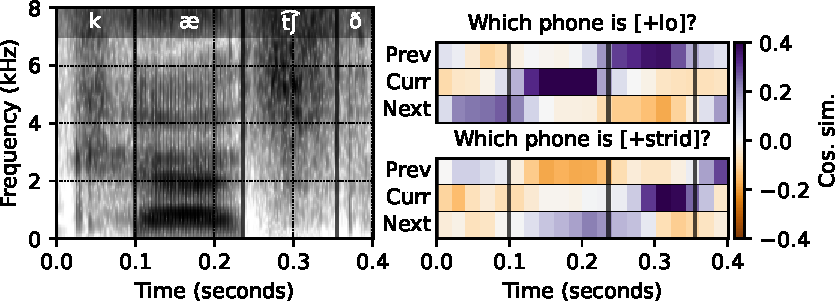
\includegraphics[width=\linewidth]{pdfs/fig1-small.pdf}
        \caption{
            Empirical demonstration of our hypothesis.
        }
        \label{fig:evidence}
    \end{subfigure}
    \caption{
        (a) Each frame-level S3M representation contains phonological vectors from position-sensitive, orthogonal subspaces.
        (b) Cosine similarity between frame-level representations and phonological vectors (\textit{low}, \textit{strident}) from the previous, current, and next phone subspaces. 
        Individual frames encode phonological information from the current and neighboring phones with respect to phonetic boundaries.
    }
    \label{fig:fig1}
\end{figure}

% https://docs.google.com/presentation/d/1hTlC2bWcDUKE7CdJ-AkUQ3MsGr8-6XUBiGVPgYj-Kr4/edit